\pagebreak
\thispagestyle{empty}
\movetoevenpage
\begin{figure}
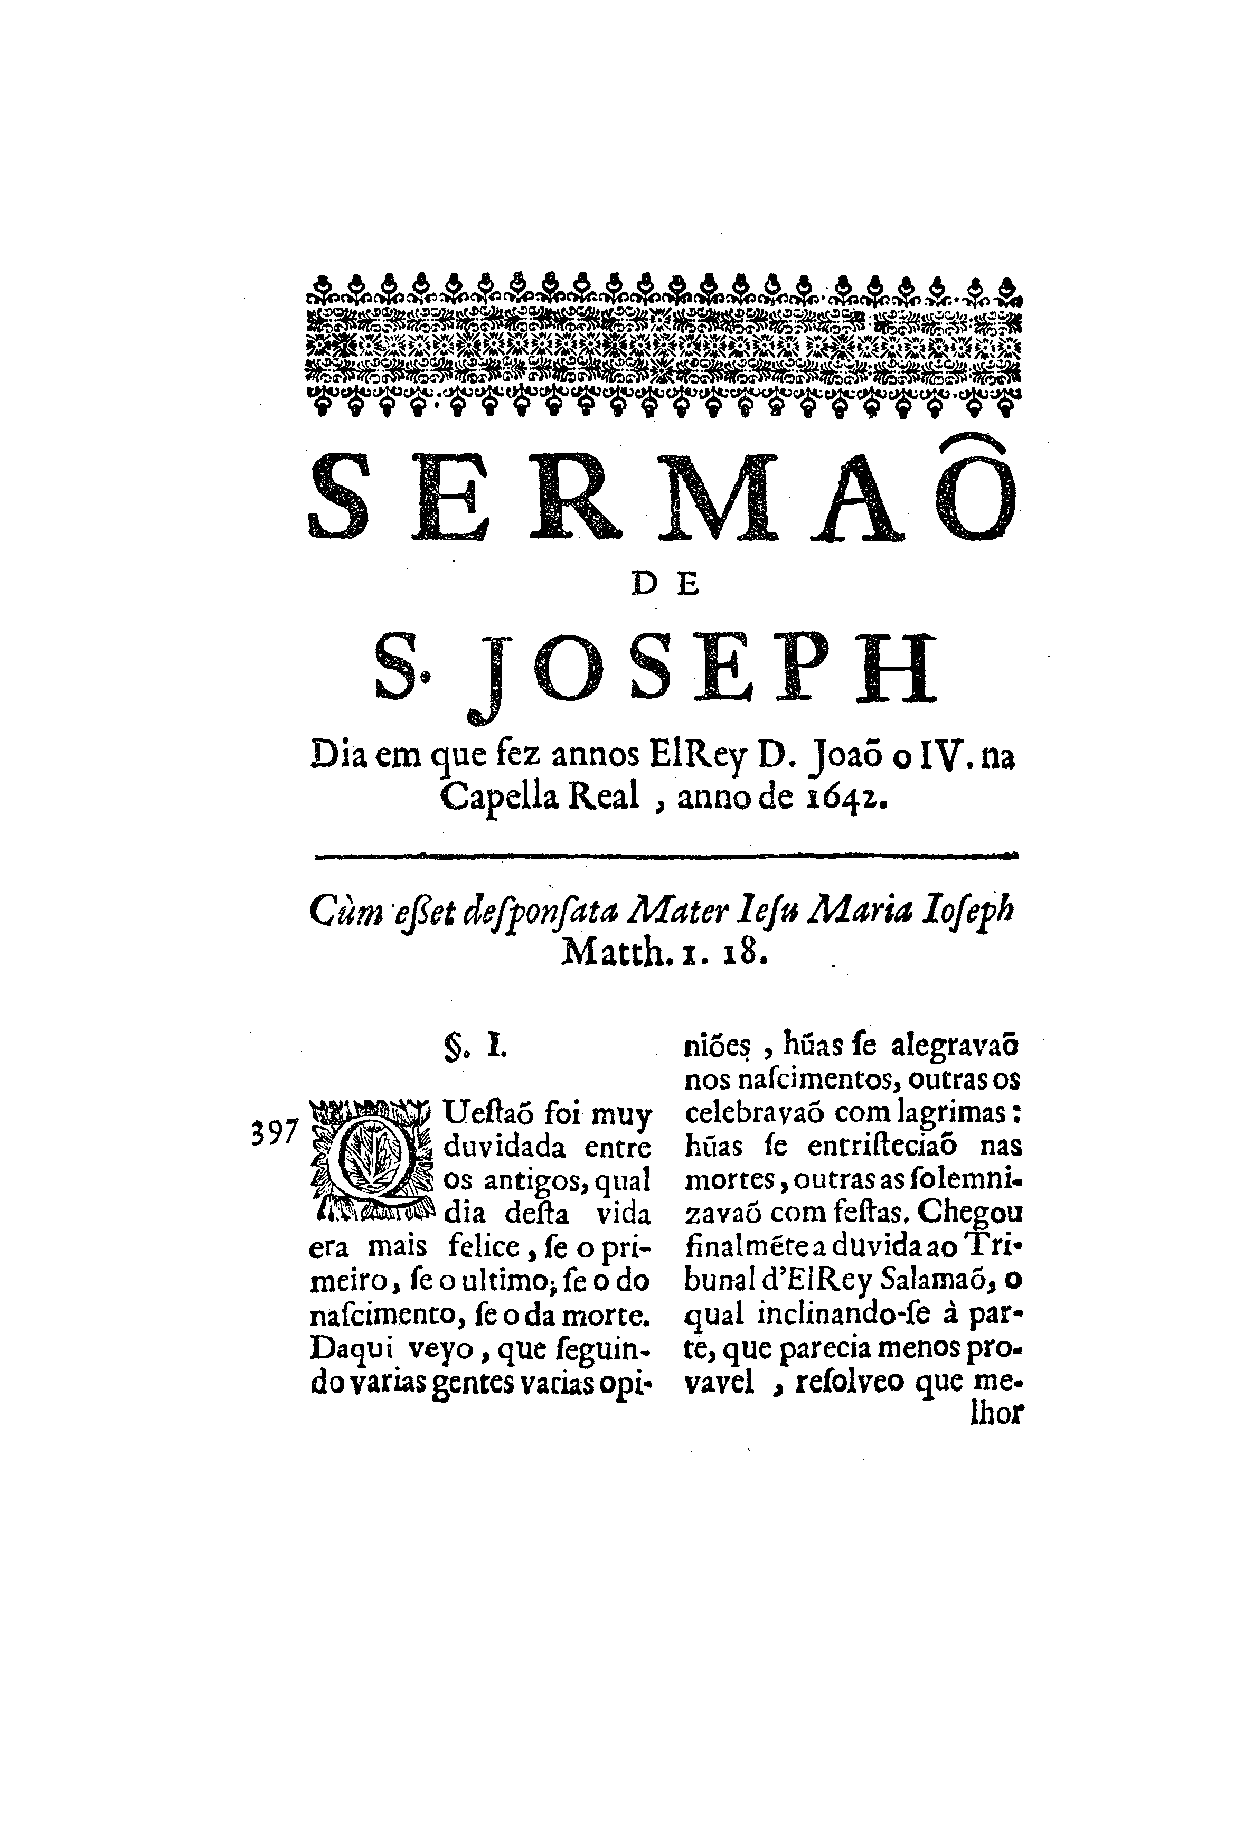
\includegraphics[width=\textwidth]{./imgs/sjose.pdf}  
\end{figure}


\chapter{Sermão de São José}

\begin{quotation}
\noindent{}Dia em que fez anos El"-Rei D.\,João o \textsc{iv} na Capela Real, ano de 1642
\end{quotation}

\epigraph{\emph{Cum esset desponsata Mater Jesu Maria Joseph.}\footnotemark}{Mt, 18.}\footnotetext{Mt 1:18 [Ora, o nascimento de Jesus Cristo foi assim: \textit{Estando Maria, sua mãe, desposada com José}, antes de se ajuntarem, achou-se ter concebido do Espírito Santo.]}

\section*{I}

\noindent{}Questão foi mui duvidada entre os antigos qual dia desta vida era mais
feliz, se o primeiro, se o último; se o do nascimento, se o da morte.
Daqui veio que, seguindo várias gentes várias opiniões, umas se
alegravam nos nascimentos, outras os celebravam com lágrimas; umas se
entristeciam nas mortes, outras as solenizavam com festas. Chegou
finalmente a dúvida ao tribunal de el"-rei Salomão, o qual, inclinando"-se
à parte que parecia menos provável, resolveu que melhor é o dia da morte
que o dia do nascimento: \emph{Melior est dies mortis die nativitatis}.\footnote{Ecl 7:2 [7:1] [\textit{Melhor é} a boa fama do que o melhor unguento, \textit{e o dia da morte do que o dia do nascimento} de alguém.]}
Com isto estar resoluto e definido assim na Escritura,
hoje parece que temos a mesma questão, ou concordada, ou ressuscitada,
porque estamos, por mercê de Deus, em um dia tão glorioso por uma morte,
tão feliz por um nascimento, que bem se pode competir dentro em si
mesmo, ou a vencer feliz suas glórias, ou a vencer glorioso suas
felicidades. Consagrou"-se este dia às glórias do céu, com a morte do
maior santo que nele reina, o divino Esposo da Virgem Maria, S.\,José, e
consagrou"-se outra vez o mesmo dia às felicidades de Portugal, com o
nascimento felicíssimo do mais desejado rei, e mais benemérito, el"-rei,
nosso senhor, Dom João o \textsc{iv}, para que sobre os trinta e oito, que hoje
conta, continue por muitos e mui compridos anos as prosperidades que
goza. Morre hoje José, e nasce Sua Majestade. Que ventura tão recíproca!
Nem José morrendo podia deixar no mundo melhor substituto, nem Sua
Majestade nascendo podia entrar no mundo com melhor planeta.

Estando Cristo, Redentor nosso, na cruz, olhou para S.\,João, o discípulo
amado, e encarregou"-lhe que tivesse cuidado de servir e acompanhar a sua
Santíssima Mãe. Reparam alguns santos em não dar o Senhor este cargo a
outro apóstolo, senão a S.\,João, porque, ainda que em São João
concorriam todas as qualidades, em algumas era igualado, e em alguma
excedido, e, para mordomo da Rainha dos Anjos, todos o excediam no
atributo da ancianidade. Pois, se era mais moço João, e havia outros
amados, e mais parentes, por
que não escolhe Cristo a outro discípulo, senão a S.\,João para este
ofício? A razão foi porque o ofício de acompanhar e servir à Senhora era
ofício de S.\,José enquanto viveu, e para substituir em ausências de
José, quem havia de ser senão João? Não é menos que de S.\,Cipriano o
pensamento: \emph{Ut non tam Joseph oneretur tanti ministerii
praepositura, sed Joannes.} Morrera José, vagara no mundo aquele
grande lugar, e para substituir em sua morte, para suceder em sua
ausência, ninguém havia no mundo que estivesse a caber, senão quem?
João, o amado de Deus. João, o amado de Deus, substitui a José:
\emph{Non tam Joseph, sed Joannes.}

E isto quando? No dia de seu nascimento. Parece que não pode ser, porque
nem o real nem o nascimento podem competir a S.\,João aqui. Ora, tudo
foi. Quando Cristo deu a S.\,João o cuidado de servir à Senhora, as
palavras que disse foram estas: \emph{Mulier, ecce filius tuus}:\footnote{Jo 19:26 [Ora, Jesus, vendo ali sua mãe e que o discípulo a quem ele amava estava presente, disse à sua mãe: \textit{Mulher, eis aí o teu filho.}]}
Mulher, eis aí teu filho.
\emph{Deinde dicit discipulo: Ecce Mater tua}:\footnote{Jo 19:27 [\textit{Depois, disse ao discípulo: Eis aí tua mãe}. Edesde aquela hora o discípulo a recebeu em sua casa.]} João, eis aí
tua Mãe. Mãe e filho, de que maneira? Mãe tinha S.\,João, mas era Maria
Salomé; filho era, mas do Zebedeu. Pois, se estes eram seus pais, como
se chama João filho da Senhora, e a Senhora mãe de João? É porque João
tornou a nascer nesta hora, e nasceu só da Virgem por força das palavras
de Cristo. Autores houve, e entre eles expressamente S.\,Pedro Damião,
que disseram que, assim como as palavras \emph{hoc est corpus
meum},\footnote{[\textit{PL}: Vol.\,14: \textit{Opera Omnia S. Petri Damiani}. Operum S. Petri Damiani in Editione Cajetani Tomus Secundus Complectens Sermones et Sanctorum Historias. Petrus Damianus: B. Petri Damiani Sanctae Romanae Ecclesiae Cardinalis, Episcopi Ostiensis, Ordinis S. Benedicti, Sermones Ordine Mensium Servato (\textsc{c,g})* Sermo \textsc{lxiv}. De Sancto Joanne Apostolo et Evangelista.]} ditas uma vez por Cristo, tiveram força para converter o
pão em corpo do mesmo Cristo, assim as palavras: \emph{Mulier, ecce
filius tuus} tiveram força para fazer a S.\,João, e o converterem de
filho do Zebedeu em filho de Maria.

De maneira que S.\,João teve dois nascimentos: um nascimento natural, com
que nasceu filho do Zebedeu; outro nascimento sobrenatural, com que
nasceu filho da Mãe de Deus. Pelo primeiro nascimento nasceu nas praias
do Tiberíades, pelo segundo nascimento nasceu ao pé da cruz. Pelo
primeiro nascimento nasceu de geração humilde, pelo segundo nascimento
nasceu da mais ilustre e real prosápia que havia no mundo, filho de uma
Senhora, herdeira de um rei morto à mão de seus inimigos: \emph{Jesus
Nazarenus, Rex Judaeorum.} Assim nasceu S.\,João segunda vez, e assim
foi necessário que nascesse, para suceder no lugar de S.\,José, como
sucedeu, porque só se pode substituir dignamente a morte de José, com
quê? Com o nascimento real de um João, o amado de Deus: \emph{Discipulum
quem diligebat: Mulier, ecce filius tuus: Non tam Joseph, sed Joannes.}

\section*{II}

Só vejo me podem reparar os curiosos em falar no dia de S.\,José por
termos de morte, sendo que mais devia, com um e outro intento,
chamar"-lhe nascimento, porque assim chama a Igreja às mortes dos santos:
\emph{Natalitia Sanctorum.} Se eu não fora mais amigo da verdade que
da propriedade, assim o fizera, mas as mortes de outros santos podem"-se
chamar nascimentos, a morte de S.\,José não. As mortes de outros santos
podem"-se chamar nascimentos, porque quando morreram à vida temporal nasceram à
vida eterna. Não assim São José. Como não estava ainda aberta a porta do
céu quando São José morreu, não foi o santo no dia de sua morte à
glória, senão ao limbo. Ao limbo São José neste dia? Valha"-me Deus, que
duvidoso horóscopo! Não sei eu como poderei provar o que entrei dizendo,
que não se podia nascer com melhor planeta. Dizem os matemáticos que nascer com
os planetas debaixo da terra é prognóstico de infelicidades.\footnote{Bocarra in Anacephaleosim Reg. lusit.}
Pois, se São José neste dia seu o temos debaixo da terra, o
corpo na sepultura, a alma no limbo, que influências podemos esperar
deste planeta em tão funesto sítio? Ora, digo que é felicíssimo auspício
ter neste nascimento a São José debaixo da terra, porque, ainda que os
planetas debaixo da terra tenham perigosas influências, tiram"-se por
exceção os planetas que são Josés: os planetas que são Josés, para
influírem felizmente, hão de estar debaixo da terra.

Estava o patriarca José em Egito; morreu, e diz o texto sagrado que
depois de sua morte cresceram muito os israelitas em número e poder:
\emph{Quo mortuo, creverunt filii Israel, quasi germinantes multiplicati
sunt: ac roborati nimis, impleverunt terram}.\footnote{Ex 1:6--7 [\textit{Sendo, pois, José falecido}, e todos os seus irmãos, e toda aquela geração, \textit{os filhos de Israel frutificaram, e aumentaram muito, e multiplicaram-se, e foram fortalecidos grandemente; de maneira que a terra se encheu deles.}]} Que os filhos de
Israel crescessem pelos merecimentos de José não me admira; antes, assim
havia de ser, que isso quer dizer José, aumento e crescimento:
\emph{Joseph accrescens.} O que me admira é que crescessem os
israelitas depois dele morto: \emph{Quo mortuo.} Se José quer dizer
crescimento, e os filhos de Israel cresceram por sua influência, por que
não cresceram em sua vida, senão depois de sua morte? A razão é porque,
para se lograrem as influências de José, há de estar debaixo da terra.
Delicadamente o tirou Hugo Cardeal do mesmo texto. Diz o texto que:
\emph{Creverunt quasi germinantes:} cresceram os filhos de Israel assim
como crescem as plantas. Bem dito, diz Hugo: \emph{Uno grano emortuo,
multa creverunt:} Cresceram os filhos de Israel como as plantas, porque,
assim como as plantas, para nascerem e crescerem, é necessário que a
virtude de que nascem se enterre primeiro debaixo da terra, assim, para
que a virtude de José influísse aumentos nos filhos de Israel, foi
necessário que ele morresse e se enterrasse primeiro: \emph{Quo mortuo,
creverunt.} Os outros planetas hão de estar em cima, mas os Josés
debaixo da terra.

Grande advertência de Filo. Pode"-se duvidar a razão por que José se
mostrou tão benigno, e fez tantos favores e mercês a seus irmãos, de
quem recebera tantos agravos. Digo que se pode duvidar, porque bem
mostraram os primeiros dois irmãos, Caim e Abel, que não basta a razão
de irmandade para abrandar corações. E se um irmão respeitado mata, um
irmão ofendido, que fará? Pois, se José estava tão ofendido de seus
irmãos, como se mostrou tão benigno e liberal com eles? A razão, disse
Filo que foi por umas palavras que disseram a José os irmãos. Quando lhe
deram conta de si, disseram que eram doze: os dez que ali estavam, um
que ficara com o pai, e outro que morrera, que era o mesmo José. As
palavras foram estas: \emph{Duodecim fratres sumus: minimus cum patre
nostro est, alius non est super}.\footnote{Gn 42 :13 [E eles disseram: Nós, teus servos, \textit{somos doze irmãos}, filhos de um varão da terra de Canaã; \textit{e eis que o mais novo está com nosso pai, hoje; mas um já não existe}.]} O menor de todos, Benjamim,
ficou com o pai; o outro, que era José, \emph{non est super:} já não
está em cima, está debaixo da terra. Já está debaixo da terra José?
Por isso se mostrou tão benigno e liberal com os irmãos, diz Filo:
\emph{Alius non est super, de se loquentes audiens, quid animi habere
potuit?} Ouvindo dizer José que já não estava em cima, senão que
estava debaixo da terra, que outra coisa pôde fazer, senão amar,
favorecer, influir beneficamente liberalidades? Os outros planetas, para
influírem benignamente hão de estar em cima; mas José, quando não está
em cima, senão debaixo da terra, como hoje (assim tem o hebreu:
\emph{Hodie non est super}) no dia em que não está em cima, senão
debaixo da terra, então influi vida, mercês, felicidades e aumentos.

\section*{III}

Temos visto o nascimento real de João, o amado, e o sítio do planeta em
que nasce, debaixo da terra, no mesmo ou semelhante dia; e, porque os
dias, como diz Davi, também se falam e se entendem uns com os outros:
\emph{Dies diei eructat verbum};\footnote{Sl 18:3 [\textit{Um dia transmite esta mensagem ao outro dia}, e uma noite comunica-a a outra noite.]} com razão perguntará o dia do
nascimento de Sua Majestade ao dia em que nasce, de São José, que
influências pode ou deve esperar de tão divino planeta. A resposta não é
como a dos matemáticos, duvidosa e incerta, mas tão certa e sem dúvida
como tudo o que dizem os evangelistas. Vamos ao nosso Evangelho, que é
de São Mateus, no capítulo primeiro, e ouçamos com admirável propriedade
o que diz, como se falara deste dia, e do nosso caso: \emph{Cum esset
desponsata Mater Jesu Maria Joseph}: Estava, diz, a Mãe de
Jesus, Maria, desposada com José. Onde se deve advertir que a palavra
desposada não significa promessa recíproca de bodas futuras, senão
verdadeiro e atual matrimônio, por contrato, e palavras de presente,
como consta do mesmo texto: \emph{Noli timere accipere Mariam conjugem
tuam}:\footnote{Mt 1:20 [E, projetando ele isso, eis que, em sonho, lhe apareceu um anjo do Senhor, dizendo: José, filho de Davi, \textit{não temas receber a Maria, tua mulher}, porque o que nela está gerado é do Espírito Santo.]} mas a cortesia do evangelista não disse casada, senão
desposada, como termo mais decente e decoroso. O que suposto, era a
Senhora já Mãe de Jesus, porque tinha concebido ao Verbo Eterno, mas
antes de mãe, primeiro desposada. E por quê? Como era e havia de ser
sempre Virgem, tanto importava ser primeiro desposada, como depois: por
que razão logo ordenou a providência divina que não concebesse ao Filho
de Deus, senão depois de desposada: \emph{Cum esset desponsata Mater
Jesu?} A razão principal é porque convinha e era necessário que a
conceição e parto da mesma Virgem estivesse encoberto: \emph{Ut
virgineus partus celaretur.} Assim o dizem São Jerônimo, São Basílio,
São João Damasceno, Santo Ambrósio,\footnote{[\textit{PL}: Vol. 16: \textit{Sancti Ambrosii Opera Omnia}. De lapsu Virginis Consecratae. Ambrosius Mediolanensis: Sancti Ambrosii Mediolanensis Episcopi de lapsu Virginis Consecratae liber Unus. (\textsc{c,g,s})* Caput \textsc{viii}.]} São Bernardo, e é comum dos santos
padres. Constava da Sagrada Escritura, pelo oráculo e testemunho do
profeta Isaías, que o Messias e rei prometido para redentor do mundo
havia de nascer de uma Virgem: \emph{Ecce Virgo concipiet, et pariet
filium}.\footnote{Is 7:14 [Portanto, o mesmo Senhor vos dará um sinal: \textit{eis que uma virgem conceberá, e dará à luz um filho}, e será o seu nome Emanuel.]} E porque este rei, não só na terra, senão no mesmo
inferno, havia de ter muitos êmulos e inimigos, esta era a importância e
necessidade por que convinha e tinha ordenado a divina Providência que
estivesse encoberto a todos, como com efeito se encobriu no desposório
ou matrimônio da Virgem Santíssima com S.\,José, parecendo que não tinha
mais mistério a conceição e nascimento daquele Filho, que o comum e
ordinário dos outros homens.

Que semelhança tem agora, ou que propriedade em São José, a providência
de Deus neste mistério com o nascimento de Sua Majestade, que Deus
guarde, no dia do mesmo santo? Disse"-o Ruperto, com umas palavras que,
se lhe pedíramos as fizesse de encomenda, não vieram mais nascida ao
intento: \emph{Ut esset sponsus, custos que Beatae Mariae Virginis, ac
nati ex ea regis:} Desposa"-se José com Maria, e nomeadamente com Maria
Mãe de Jesus, porque o fim destes desposórios foi ser José esposo da
Virgem, e guarda do rei
nascido: \emph{Custos nati regis}. Oh! grande excelência! Oh! grande
glória! Oh! dignidade superior a todos os santos a de José! Que os foros
da mesma onipotência nasçam debaixo de seu amparo, e que, não tendo
Cristo anjo da guarda, porque é Deus, tenha por custódio um homem, que é
São José: \emph{Custos nati regis!}\footnote{[\textit{PL}: Vol. 167 Col. 1540A: \textit{Opera Omnia Ruperti Tuitiensis}. Rupertus Tuitiensis: R.D.D. Ruperti Abbatis Tuitiensis de Trinitate et Operibus Ejus libri \textsc{xlii}. R.D.D. Ruperti Abbatis Tuitiensis De Trinitate et Operibus Ejus libri \textsc{xlii}. In VaI. Quatuor Evangelistarum Commentariorum liber Unus. Caput \textsc{vi}. Quod in eadem generatione tres isti Abraham, David, et joseph, magis insignes sint, et quod ad istos per incrementa ternaria promissio Christi facta sit. Caput \textsc{vi}.]} Grande glória de José, e grande
graça também do nosso rei e reino! Que o amasse Deus, e cuidasse do seu
remédio com tão especial providência, que o patrocínio que deu em seu
nascimento ao rei que havia de restaurar o mundo, esse mesmo patrocínio
desse em seu nascimento ao rei que havia de restaurar a Portugal! Um e
outro nasceu debaixo da mesma proteção, um e outro nasceu debaixo da
tutela e amparo de São José: \emph{Joseph, custos nati regis.}

Sendo, pois, estes dois reis nascidos ambos reis, ambos redentores e
ambos encobertos, o primeiro, como diz a profecia de Isaías: \emph{Vere
tu es Deus absconditus, Deus Israel Salvator}:\footnote{Is 45:15 [\textit{Verdadeiramente, tu és o Deus que te ocultas, o Deus de Israel, o Salvador.}]} O segundo,
prometido pela profecia e; tradição de Santo Isidoro a Espanha, não com
outro nome ou antonomásia„ senão a do Encoberto, vejamos quão
particularmente encobriu a um e outro o que a um e outro deu Deus por
guarda o cuidado e vigilância de São José. A Cristo encobriu"-o como
Esposo de Maria, nove meses e treze dias, desde suar conceição até
depois de seu nascimento, em que o descobriu a estrela no Oriente, aos
Magos, e os Magos, em seguimento dela, a toda Judeia. E como o encobriu
\emph{Spiritus sanctus superveniet in te, et virtus Altissimi obumbrabit
tibi.} A Virgem, Senhora nossa, tinha dois esposos, um divino,
outro humano. O esposo divino era o Espírito Santo; o humano, São José.
Do primeiro esposo era obrai o filho concebido, como disse o anjo à
mesma Virgem: \emph{Spiritus Sanctus superveniet in te}: acrescentando:
\emph{Et virtus Altissimi obumbrabit tibi:}\footnote{Lc 1:38 [Lc 1:35] [E, respondendo o anjo, disse-lhe: O Espírito Santo descerá sobre tí, e \textit{a virtude do altíssimo te cobrirá com a sua sombra}. E, por isso mesmo, o santo, que há de nascer de ti, será chamado Filho de Deus.]} que ar virtude do Altíssimo
lhe faria sombra. E que sombra foi esta? Ou quem foi esta sombra? Foi
sem dúvida o segundo esposo, a cuja sombra esteve a Virgem depois de
desposada, e, com a sombra e nome de pai, encobriu o que verdadeiramente
não era seu filho. Assim ficou o rei e Redentor, que havia de ser do
mundo, encoberto desde sua encarnação nove meses até seu nascimento e
treze dias, até que a estrela, e os Magos, e Deus por eles, o descobriu
ao mundo: \emph{Ubi est qui natus est rex Judaeorumt?}\footnote{Mt 2:2 [E perguntaram: \textit{Onde está aquele que é nascido rei dos judeus?} Porque vimos a sua estrel no Oriente e viemos a adorá-lo.]}

Mas, se São José guardou encoberto a Cristo nove meses e treze dias, que
comparação tem este tempo, que não chega a um ano, com mais de trinta e
seis anos inteiros em que teve encoberto ao rei encoberto de Portugal,
desde o dia do seu nascimento até o felicíssimo de sua restituição? Vejo
que me respondem que São José não só encobriu a Cristo naquele primeiro
ano não acabado, mas em outros, cujo número certo se não sabe. Sabendo
pelo anjo que Herodes, entre os inocentes de Belém, queria tirar a vida
a Cristo, fugiu da Judeia para o Egito, e, depois da morte do mesmo
Herodes, sabendo, também por aviso do céu, que reinava em Judeia
Arquelau, seu filho, retirou"-se para Galileia. De sorte que, para
encobrir o primeiro rei nascido, tomou por meio tirá"-lo diante dos olhos
dos dois reis seus inimigos, e escondê"-lo em terras estranhas.
Porém, para encobrir o segundo rei, não só no seu nascimento, nem na sua
infância, puerícia ou adolescência, senão na idade de varão perfeito em
tantos anos, a traça com que o encobriu a outros dois reis, que não
menos lhe podiam tirar a vida e a coroa, qual seria? Verdadeiramente
milagrosa e digna da onipotência divina. Dentro na mesma Espanha, dentro
no mesmo Portugal, e diante dos olhos dos mesmos reis, escondeu e
encobriu de maneira ao encoberto que, vendo"-o, o não viam nem viram. É
certo que assim foi, mas duvidoso, como podia ser.

No dia da Ressurreição, ajuntou"-se Cristo aos dois discípulos que iam
para Emaús, os quais em todo aquele caminho o viam e ouviam, sem o
conhecerem. Porventura transfigurou"-se Cristo, ou mudou as feições do
rosto? Por nenhum modo. Pois, se eram seus discípulos, costumados a
vê"-lo todos os dias, e agora o estavam vendo, e no seu rosto não havia
mudança, como o não conheciam? Responde o evangelista: \emph{Oculi eorum
tenebantur ne eum agnoscerent}.\footnote{Lc 24:16 [\textit{Mas os olhos deles estavam como que fechados, para que o não conhecessem}.]} A palavra \emph{tenebantur}
melhor se pode entender do que declarar na nossa língua:
\emph{tenebantur,} estavam detidos; \emph{tenebantur,} estavam presos;
\emph{tenebantur,} estavam suspensos; \emph{tenebantur,} estavam em si e
fora de si, como extáticos, os olhos que o viam, e não conheciam.
Fazendo este milagre nos discípulos a onipotência de Cristo, e nos reis,
que tanto podiam temer e acautelar"-se do que hoje é nosso, a mão
invisível de São José.
Desde o princípio, em que se fizeram senhores de Portugal aqueles reis
estranhos, Filipe \textsc{ii} tinha diante dos olhos a senhora D.\,Catarina,
Filipe \textsc{iii} ao Duque D.\,Teodósio, Filipe \textsc{iv} a Sua Majestade, que,
finalmente, lhe tirou da cabeça a coroa, e, vendo"-os, não conheciam o
que neles deviam recear e temer, cegando"-os São José com a mesma luz de
seus olhos, encobrindo o seu e o nosso Encoberto com o descobrir.

Assim desempenhou o grande santo a obrigação que tinha de encobrir e
provar o nome de encoberto no novo rei nascido no seu dia; mas ainda lhe
falta, ou nos falta, uma maior consideração e vigilância deste seu
empenho. O ódio, a emulação, a cautela, o receio de perder o ganhado em
Portugal, que tinham os reis estranhos, a grandeza do poder e a doçura
do possuir, podia lisonjear e adormecer todo este cuidado; mas da nossa
parte, e em nós, os portugueses, além da dor do perdido, estava com os
olhos abertos ao remédio o amor, o desejo e a necessidade. O amor, ainda
que é cego para ver, é lince para adivinhar; o desejo é um afeto sempre
ardente e inquieto, que não sabe sossegar um momento; sobretudo, a
necessidade da redenção, da liberdade, e de rei natural, era a que mais
apertava os cordéis a este tormento, e tinha com a soga na garganta
todos estes afetos. E como podia ser que, sendo eles tão vigilantes, e
tendo sempre o direito da corroa, e a pessoa do rei a quem pertencia
diante dos olhos, de tal sorte a encobrisse S.\,José, que a ninguém
viesse ao pensamento ser ele o que o havia de recuperar? Mas em encobrir
o nosso Encoberto neste grande perigo de o declararem as evidências ou
conjecturas de alguns destes afetos, mostrou o santo quão alta e
delicadamente observou as obrigações do ofício de o guardar:
\emph{Custos nati Regis}; equivocando milagrosamente um rei com outro
rei, e encobrindo um vivo com outro morto. Perdeu"-se, ou morreu, na
batalha de África el"-rei Dom Sebastião, e puderam tanto as saudades de
um rei, que se tinha perdido a si e a nós, que, sem se divertirem aonde
deviam, deram em esperar dele, e por sua vida e vinda, a nossa redenção,
e este foi o altíssimo conselho com que São José, debaixo das cinzas do
rei passado e morto, conservou e teve encoberto o rei futuro e vivo. Não
vemos conservar"-se vivo o fogo, debaixo das cinzas que o encobrem? Pois,
assim conservou e encobriu São José a vida de el"-rei, que Deus guarde,
debaixo das cinzas de el"-rei D.\,Sebastião defunto. É o que diz
expressamente Isaías no capítulo 61. Promete Deus ali de alegrar os
tristes, de consolar os desconsolados, de libertar os cativos, e conclui
que pelas cinzas lhe dará a coroa: \emph{Ut mederer contritis corde, et
praedicarem captivis indulgentiam: ut consolarer omnes lugentes};\footnote{Is 61 :1-3 [O espírito do Senhor repousou sobre mim, porque o Senhor me ungiu; ele me enviou para evangelizar os mansos, \textit{para curar os contritos de coração, e pregar a redenção aos cativos}, e a liberdade aos encarcerados; para publicar o ano da reconciliação do Senhor, e o dia da vingança do nosso Deus, \textit{para consolar todos os que choram}; para conceder \textit{e dar} aos de Sião, que choram, \textit{uma coroa em vez de cinza}, óleo de gozo em vez de pranto, um vestido de glória em troca de seu espírito de aflição; e os que habitarem nela serão chamados fortes na justiça, plantas do Senhor para lhe darem glória.]} e
finalmente: \emph{Et darem eis coronam pro cinere.} Assim
estava Portugal triste, assim estava desconsolado, assim estava cativo,
e assim lhe prometia São José a coroa perdida, debaixo das cinzas do rei
morto reputado por vivo, e assim conservava vivo e encoberto aquele que
verdadeiramente havia de
restituir aos tristes, desconsolados e cativos a coroa perdida. De
maneira que, encoberta a verdade debaixo do engano, a esperança debaixo
da desesperação, a vida debaixo da morte, e a coroa debaixo das cinzas,
aos príncipes estranhos, que tudo isto tinham por riso, não lhes dava
cuidado, o remédio; e os vassalos, amigos e naturais, que o tinham,
pouco menos, quase por fé, com milagrosa providência, enganada a sua
dor, e o seu amor, o seu desejo e a sua necessidade, se consolavam e
animavam da falsa e equivocada esperança, até que a verdade, debaixo
dela encoberta, ao tempo destinado pelo céu, lhe trouxe a felicidade que
hoje logramos.

\section*{IV}

Certo que ponderar cabalmente esta felicidade será causa de não faltar
nunca Portugal ao eterno agradecimento a São José. Que uma vida (não
sejamos ingratos, por não saber o que devemos a Deus) que uma vida, em
que estavam fundadas as consequências que hoje se logram, apesar da
emulação de dois reis, debaixo de sua mesma jurisdição se conservasse!
Que nasça a décima"-sexta geração de Portugal tão esperada, e que, sendo
décima"-sexta por três vias, nem o amor dos naturais, nem os ciúmes dos
estranhos em trinta e sete anos o descobrisse! Vivo, apesar de tantas
advertências políticas; encoberto, apesar de tantas evidências
manifestas! Grandes milagres da providência divina, e este segundo, a
meu ver, ainda maior. E, se não, pergunto: Qual foi a razão por que
ordenou Deus que o Libertador que havia de ser de Portugal se conhecesse
tantos anos antes no mundo, não pelo nome de Libertador, senão pelo nome
de Encoberto? A razão foi porque maior milagre da Providência era
conservá"-lo encoberto, que fazê"-lo libertador. Fazê"-lo libertador, foi
deliberarem"-se os homens a uma coisa muito útil; conservá"-lo encoberto,
foi cegarem"-se os homens a uma coisa muito manifesta; e maior milagre é
encobrir evidências ao entendimento, que persuadir conveniências à
vontade. O que todos ponderam, o que todos admiram, o de que todos fazem
maior caso, é que se unissem e concordassem as vontades de todo um
reino, para fazer o que fizeram. Muito foi, mas, bem considerado, não
foi muito, porque, que muito que as vontades dos homens se persuadissem
a uma coisa tão útil e tão honrosa, como ter reino, ter rei, ter
liberdade, viver sem cativeiro e sem opressão? Porém, que o autor
felicíssimo de todo este bem nascesse e vivesse entre nós tão retratado
pelos oráculos divinos e ainda nomeado pelo próprio nome, e o tivesse
Deus encoberto, sem que o amor nem a emulação, que são os dois afetos
mais linces, o descobrissem! Que o vissem os olhos, e que guardasse
segredo o entendimento! Que suspirassem os desejos, e que não bastassem
as maiores advertências! Dissimulado a evidências, e encoberto a olhos
vistos! Este é o maior milagre, esta a maior maravilha, mas agora
exercitada, e muitos séculos antes já ensaiada: por quem? Pelo autor da
mesma proteção, São José.

Conta o texto sagrado, no quarto Livro dos Reis, capítulo onze, que em
uma ocasião quiseram tirar a vida tirânica os herdeiros do sangue real
de Israel ao menino Joás; porém, que Josabá o livrou do perigo, e o
criou escondidamente:
\emph{Abscondit eum, ut non interficeretur},\footnote{4Rs 11:2 [Mas Jeoseba, filha do rei Jeorão, irmã de Acazias, tomou a Joás, filho de Acazias, e o furtou dentre os filhos do rei, aos quais matavam, e o pôs, a ele e à sua ama, na recâmara, e \textit{o escondeu} de Atalia, \textit{e assim não o mataram}.]} até que, passados
alguns anos, os nobres do povo se uniram, e todos com as armas nas mãos
entraram no paço real, e, impedindo as guardas em um sábado, aclamaram
por rei a Joás, e o meteram de posse do reino que lhe pertencia,
lançando do paço a Atália, uma senhora que então governava. Desta
maneira refere o texto este caso, e bem se vê que é tão próprio do que
sucedeu em Portugal que, se ao nome de Joás se mudara o \emph{s} em \emph{m},
se pudera trasladar este capítulo, e escrever"-se em nossas crônicas. Bem
está: mas quem fez isto? A quem se deve esta façanha? Quem há de levar a
glória desta maravilha? Quem? São José. Diz Isidoro Isolano que Josabá,
a cuja indústria deve sua vida e restituição Joás, foi figura de São
José, esposo da virgem: \emph{Joseph profecto in Jozaba praefiguratus
est, quae Joas infantem clam nutrivit et aluit, ac regem Israel tandem
constituit.} Hei de construir as palavras ao pé da letra, para maior
glória de São José, e maior evidência do nosso caso. \emph{Joseph
profecto in Jozaba praefiguratus est}. Verdadeiramente São José foi
figurado e representado em Josabá: \emph{Quae Joas infantem clam
nutrivit et aluit:} que guardou ao infante Joás vivo e encoberto:
\emph{Ac regem Israel tandem constituit:} e, finalmente, o fez rei de
Israel, metendo"-o de posse do reino que lhe tocava. E não é isto mesmo
o que fez São José com o rei e reino de Portugal? Nem o caso pode ser
mais próprio, nem eu quero dizer mais nesta matéria.

Estas são as obrigações em que São José tem empenhado a Vossa Majestade,
senhor, e as consequências delas são que, assim como São José não só foi
salvador do Salvador, senão também do mundo, assim não foi só salvador
do nosso libertador, senão também do reino libertado. Espero em Deus que
o he de provar literalmente. \emph{Benedictio illius qui apparuit in
rubo, veniat super caput Joseph}:\footnote{Dt 33:16 [E com o mais excelente da terra, e com a sua plenitude, e \textit{com a benevolência daquele que habitava na sarça, a bênção venha sobre a cabeça de José} e sobre o alto da cabeça do que foi separado de seus irmãos.]} A bênção daquele que
apareceu na sarça desça sobre José. Esta bênção foi lançada ao
patriarca José, e diz o Pelusiota, e outros, que se cumpriu em São José,
Esposo da Virgem. E qual foi a bênção daquele que apareceu na sarça a
Moisés? Ele mesmo o disse: \emph{Vidi afflictionem populi mei, et
descendi ut liberem eum}:\footnote{Ex 3:7-8 [E disse o Senhor: \textit{Tenho visto atentamente a aflição do meu povo}, que está no Egito, e tenho ouvido o seu clamor por causa dos seus exatores, porque conheci as suas dores. \textit{Portanto, desci para livrá-lo} da mão dos egípcios e para fazê-lo subir daquela terra a uma terra boa e larga, a uma terra que mana leite e mel; ao lugar do cananeu, e do heteu, e do amorreu, e do ferezeu, e do heveu, e do jebuseu.]} Vi a aflição de meu povo, debaixo
do poder de um rei estranho, e desci do céu a libertá"-lo. Pois, se a
bênção do que apareceu a Moisés na sarça é ser libertador do povo
oprimido do poder de um rei estranho, e esta bênção se cumpriu em São
José, Esposo da Virgem, digam"-me agora os historiadores quando se
cumpriu esta bênção, senão na restauração de Portugal. Viu o santo as
aflições deste povo verdadeiramente seu, e desceu do céu a libertá"-lo,
guardando com particular providência a vida do nosso felicíssimo
libertador, como fez à de Cristo, segundo a proteção que tomou em um e
outro nascimento: \emph{Custos nati regis}, que foi o fim com que se
desposou com a Virgem: \emph{Cum esset desponsata Mater Jesu Maria
Joseph.}

\section*{V}

Tenho acabado o sermão: de todo ele quisera tirar somente uma coisa,
queira o Senhor seja tão bem recebida nos ânimos de todos, como é a
todos necessária e importantíssima. O que concluo de todo este discurso
é que deve o Reino de Portugal tomar solenemente a São José por
particular advogado, e protetor de sua conservação e aumentos. A razão que tenho
para isto é a mais eficaz que pode ser: querer Deus que seja assim, nem
nós devemos querer outra coisa. Sonhou el"-rei Faraó que haviam de vir a
seu reino aqueles catorze anos de vária fortuna, e dizendo"-lhe que
importava prevenir"-se de algum varão de grande prudência, que
superintendesse à conservação e remédio do reino: \emph{Placuit Pharaoni
consilium},\footnote{Gn 41:36 [41 :37] [\textit{Agradou o conselho a Faraó} e a todos os seus ministros.]} contentou o conselho ao rei, e voltando"-se
para José, disse: \emph{Numquid sapientorem et consimilem tui invenire
potero}?\footnote{Gn 41:39 [Depois, disse Faraó a José: Pois que Deus te fez saber tudo isto, \textit{ninguém há tão inteligente e sábio como tu.}]} Porventura, José, posso eu achar algum que seja mais
sábio, mais prudente, e em cujas mãos e conselho esteja mais segura
minha monarquia? O cetro e a coroa ponho debaixo do vosso patrocínio:
mandai, ordenai, despendei não como vassalo, mas como pai. O mesmo digo
no nosso caso.

Isidoro de Isolanis, já acima alegado, autor que há muitos anos que
escreveu, admirando"-se muito de que em seu tempo não fosse celebrado na
Igreja o glorioso São José, conclui assim: \emph{Suscitabit Dominus
Sanctum Joseph ad honorem nomini sui, caput et patronum peculiarem
Imperii militantis Ecclesiae:} Esteja embora esquecido por agora São
José, e não seja sua memória tão celebrada como merece, que Deus
levantará este grande santo a seu tempo, para que seja particular
padroeiro do seu império na Igreja, militante: \emph{Patronum peculiarem
Imperii militantis Ecclesiae.} Duas coisas havemos de saber para
entendimento destas palavras: uma, quando se começou a celebrar São
José; outra, qual é no mundo o império de Cristo. O tempo em que se
começou a celebrar São José foi pontualmente depois da perda de el"-rei
Dom Sebastião, de triste memória, e antes da felicíssima restituição à
coroa de el"-rei Dom João, nosso Senhor, para que, posto entre a ruína do
reino e o remédio, compadecido da ruína, a remediasse. E o império de
Cristo, qual é? O mesmo Senhor foi servido de no"-lo explicar quando
disse a nosso fundador, o senhor rei Dom Afonso Henrique: \emph{dolo in
te, et in semine tuo imperium mihi stabilire:} Quero em vós, e em vossa
descendência, estabelecer o meu império. Pois, se Deus levanta no
mundo a São José, quando quer levantar a Sua Majestade por rei, se o
império de Cristo na Igreja militante somos nós, e São José há de ser
particular padroeiro deste império, que resta, senão que efetivamente se
conclua de nossa parte, que é o constituir e reconhecer com pública
solenidade a São José por protetor particular do Reino de Portugal, e
sua conservação, dizendo a este José o que os egípcios disseram ao
outro: \emph{Salus nostra in manu tua est: respiciat nos tantum Dominus
noster, et laeti serviemus Regi?}\footnote{Gn 47:25 [E disseram: \textit{A vida nos tens dado; achemos graça aos olhos de meu senhor e seremos servos de Faraó.}]}


